\documentclass{report}
\usepackage[T1]{fontenc} % Fontes T1
\usepackage[utf8]{inputenc} % Input UTF8
\usepackage[backend=biber, style=ieee]{biblatex} % para usar bibliografia
\usepackage{csquotes}
\usepackage[portuguese]{babel} %Usar língua portuguesa
\usepackage{blindtext} % Gerar texto automaticamente
\usepackage[printonlyused]{acronym}
\usepackage{hyperref} % para autoref
\usepackage{graphicx}
\graphicspath{ {imagens/} }

\bibliography{bibliografia}


\begin{document}
%%
% Definições
%
\def\titulo{Sistemas operativos}
\def\data{06/12/2020}
\def\autores{Bruno Gomes, João Artur}
\def\autorescontactos{(103320) brunofgomes@ua.pt, (nmec2) autor2@ua.pt}
\def\versao{VERSAO}
\def\departamento{Departamento de Eletrónica, Telecomunicações e Informática}
\def\empresa{Universidade de Aveiro}
\def\logotipo{ua.pdf}
%
%%%%%% CAPA %%%%%%
%
\renewcommand{\contentsname}{Índice}
\begin{titlepage}

\begin{center}
%
\vspace*{50mm}
%
{\Huge \titulo}\\ 
%
\vspace{10mm}
%
{\Large \empresa}\\
%
\vspace{10mm}
%
{\LARGE \autores}\\ 
%
\vspace{30mm}
%
\begin{figure}[h]
\center
\includegraphics{\logotipo}
\end{figure}
%
\vspace{30mm}
\end{center}
%
\begin{flushright}
\versao
\end{flushright}
\end{titlepage}

%%  Página de Título %%
\title{%
{\Huge\textbf{\titulo}}\\
{\Large \departamento\\ \empresa}
}
%
\author{%
    \autores \\
    \autorescontactos
}
%
\date{\data}
%
\maketitle

\pagenumbering{roman}

%%%%%% RESUMO %%%%%%
\begin{abstract}
O principal objetivo deste trabalho visa a mostrar os diferentes tipos de sistemas operativos que têm vindo a ser criados ao longo do tempo. Vamos introduzir o conceito de 'sistema operativo', para dar um noção geral do que vai ser falado neste trabalho. Iremos falar do Windows, Linux, IOS e macOS. Basicamente vamos falar da história e evolução de cada um, e como têm contribuido para a evolução do meio em que vivemos hoje. Adicionalmente, este trabalho pretende mostrar as diferentes funcionalidades e potencialidades menos evidentes que tenham passado despercebidas pelos utilizadores, de cada um dos sistemas operativos que irão ser falados. Anexamente, este trabalho pretende evidenciar a inovação, e facilidade de acesso a um panóplia de conteúdos e ferramentas que têm vindo a facilitar a vida de praticamente toda a população mundial, e que de certa forma tem vindo a criar uma certa dependência, nas pessoas que os usam, devido ao facto de o sistema operativo ser um ferramenta poderosa, e essencial nos computadores dos dias de hoje. Também iremos falar da utilização de 'virtual boxes', que são utilizadas para simular ambientes de trabalho de um sistema operativo escolhido pelo utilizador, dentro do sistema operativo originalmente instalado na sua máquina. Para concluir este resumo, qualquer pessoa que esteja interessada em saber mais sobre sistemas operativos, pode consultar este trabalho, pois desta maneira ficará a ter uma ideia geral do assunto.
\end{abstract}

%%%%%% Agradecimentos %%%%%%
% Segundo glisc deveria aparecer após conclusão...
\renewcommand{\abstractname}{Agradecimentos}
\begin{abstract}
Eventuais agradecimentos.
Comentar bloco caso não existam agradecimentos a fazer.
\end{abstract}


\tableofcontents
% \listoftables     % descomentar se necessário
% \listoffigures    % descomentar se necessário


%%%%%%%%%%%%%%%%%%%%%%%%%%%%%%%
\clearpage
\pagenumbering{arabic}

%%%%%%%%%%%%%%%%%%%%%%%%%%%%%%%%
\chapter{Introdução}
\label{chap.introducao}

Para começar, podemos afirmar que maior parte da população sabe para que serve um sistema operativo, mas o que é um sistema operativo ao certo?

Basicamente, um sistema operativo consiste num conjunto de programas que permite criar uma interface entre o computador e o usuário do mesmo, ou seja permite gerenciar vários recursos do computador, tais como a memória, definição de processos que precisam de mais atenção do CPU ou GPU, o sistema operativo também permite ao usuário criar um sistema de arquivos para guardar qualquer tipo de documentos que o usário queira, criando desta forma um ambiente de trabalho fácil de organizar e navegar. Resumindo e concluindo é o sistema operativo que permite a comunicação entre a máquina e o utilizador da mesma.

\vspace{5mm} %5mm vertical space

No entanto há que notar, que um sistema operativo não é uma unidade única, isto significa que este é constituído por diversas partes que permitem o funcionamento da relação entre o sistema e o computador.

Portanto as componentes mais importantes de um sistema operativo são:

\vspace{5mm} %5mm vertical space

\begin{itemize}
    \item Kernel;
    \item Rede;
    \item Segurança;
    \item Shell;
\end{itemize}

\vspace{5mm} %5mm vertical space

O \textbf{Kernel} (em português núcleo), possui um papel extremamente importante no funcionamento do computador. Pois é o Kernel que estabelece a ligação entre o processamento de dados e os programas, ou seja podemos afirmar que o kernel desempenha a função de "cérebro" do computador. Também devemos salientar que o kernel do linux tem ganho bastante notoriedade, devido ao facto de este ser usado em praticamente todos os sistemas operacionais Android para Tablets, Smartphones e Smartwatches, no entanto ambos o Windows e o macOS possuem um kernel.

\vspace{5mm} %5mm vertical space

A \textbf{rede} também é uma parte fundamental de um sistema operativo, pois só assim é possível estabelecer ligações com outros computadores, servidores e outros dispositivos. Ou seja, isto permite a conexão de computadores com sistemas operativos diferentes através da mesma rede, permitindo desta forma a partilha de diversos recursos sejam estes impressoras ou scanners por exemplo.

\vspace{5mm} %5mm vertical space

Praticamente todos os sistemas operativos já vêm com aplicações que asseguram a \textbf{segurança} do computador, temos o exemplo da firewall do Windows que já tem vindo a ser implementada desde 2001 (ano em que o Windows XP foi criado), existe também o Windows Defender cuja função principal é defender o computador de alterações no sistema causadas por softwares indesejados, adicionalmente também serve para remover malwares, spywares, trojans e adwares instalados na máquina.

Ainda podemos referir os sistemas de encriptação que são usados para codificar certos dados que só podem ser acedidos, sabendo uma palavra-passe, isto faz com que o acesso á informação seja restrito apenas ás entidades que saibam a cifra para aceder ao conteúdo.

\vspace{5mm} %5mm vertical space

Finalmente temos a \textbf{Shell} (casca), que se trata de uma camada mais superficial do núcleo (kernel) do sistema operativo, que foi falado logo no primeiro ponto.

Resumidamente, a Shell estabelece uma comunicação direta entre o usuário e o sistema operativo que ele opera, a partir desta comunicação é possível fazer invocações ao sistema operativo tais como invocar vários tipos de programas através de uma linha de comandos, o utilizador tem de ser um pouco curioso e procurar um prompt para introduzir esses comandos. Devemos salientar que existe uma variadade extraordinária de comandos disponíveis para serem usados, todos eles com funcionalidades diferentes.

Cada utilizador de um certo sistema operativo tem uma shell dedicada á sua conta, isto que dizer que é disponibilizada uma shell a um utilizador sempre que ele efetue o login na mesma.

Para concluir, deve-se referir que não existe só um tipo de shell, o Windows tem a "Windows Shell" que é uma shell gráfica, também existe a Bourne Shell que é a mãe de todas as shells dos sistemas UNIX que também são usadas nos sistemas operativos mac OS.  

\vspace{5mm} %5mm vertical space

Dito isto, de que forma é que o computador "executa" o respetivo sistema operativo?

É uma operação bastante simples, portanto o computador recorre ao auxílio de um programa armazenado em uma memória não-volátil ROM denominado de "BIOS", isto tudo é executado num processo chamado "bootstrapping", que é um processo autossustentável, ou seja é um processo que não precisa de um fator externo para ser executado.

Após a BIOS executar testes para garantir que tudo é iniciado de uma forma ordeira e sem erros, incluindo monitores, discos e outros componentes do computador, o BIOS começa a procurar pelo sistema operativo nas unidades de armazenamento do computador, como por exemplo no disco rígido, de seguida o sistema operativo começa a comandar a máquina.

A partir daqui, correm outros programas que asseguram o bom funcionamento do sistema operativo, para evitar a corrupção de ficheiros e eventualmente a corrupção do sistema inteiro.

\vspace{5mm} %5mm vertical space

Para finalizar, existem duas maneiras de abordar o assunto de funcionamento de um sistema operativo:

\begin{itemize}
    \item visão de cima para baixo (\textbf{top-down}): o sistema operativo age como uma "secção" que fica entre o hardware e o utilizador, fornecendo ao utilizador uma forma mais amigável de interagir com a máquina, através de sistemas de janelas, por exemplo;
    \item visão de baixo para cima (\textbf{bottom-up}): nesta situação o sistema operativo é que faz a gestão do hardware da máquina, isto é, controla a quantidade de memória alocada para o funcionamanento de um software do usuário, assim como também o controlo dos dispositivos de entrada e saída (rato, teclado, impressoras...);
\end{itemize}

\begin{figure}[h!]
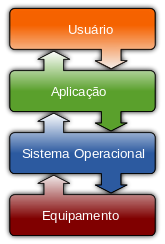
\includegraphics[width=0.4\textwidth]{img_so.png}
\centering
\caption{Representação da visão "top-down" e "bottom-up".}
\end{figure}

\chapter{Microsoft}
\label{chap.microsoft}
Descreve os métodos utilizados para obtenção de resultados.

Neste esqueleto de relatório aproveitamos este capítulo para exemplificar
como se usam alguns elementos de {\LaTeX}.

\section{História da Microsoft}

A Microsoft foi fundada no dia 4 de Abril de 1975, por Bill Gates e Paul Allen, na cidade de Albuquerque no estado "New Mexico".

A empresa Microsoft (incialmete chamada "Micro-Soft"), foi fundada com o a finalidade de produzir software para o primeiro microcomputador desenvolvido, o "Altair 8800". Para se dedicarem inteiramente á sua empresa, Paul Allen
demite-se do seu trabalho como programador em Boston, e Bill Gates decide sair da universidade de Harvard onde andava a estudar direito, isto deve-se ao facto de a empresa ser sediada em Albuquerque, pois foi lá que foi desenvolvido o computador "Altair 8800" numa outra empresa chamada MITS.

Gates e Allen propuseram criar um interpretador para o computador que tornasse possível a leitura da linguagem de programação "BASIC", de forma a tornar a máquina mais eficiente e capaz na realização de diversas tarefas.

Com a ajuda de Monte Davidoff,
\subsection{Utilização de acrónimos}
\label{sec.util}
Esta é a primeira invocação do acrónimo \ac{ua}.
E esta é a segunda: \ac{ua}.


Outras duas referências a \ac{miect}
e \ac{miect}.

\subsection{Referências bibliográficas}
Informação relativa à estrutura formal de um relatório pode ser obtida
na página do \ac{glisc}\cite{glisc}.

Como foi apresentado na \autoref{sec.util}...

\chapter{Resultados}
\label{chap.resultados}
Descreve os resultados obtidos.

\chapter{Análise}
\label{chap.analise}
Analisa os resultados.

\chapter{Conclusões}
\label{chap.conclusao}
Apresenta conclusões.

\chapter*{Contribuições dos autores}
Resumir aqui o que cada autor fez no trabalho.
Usar abreviaturas para identificar os autores,
por exemplo AS para António Silva.
No fim indicar a percentagem de contribuição de cada autor.

%%%%%%%%%%%%%%%%%%%%%%%%%%%%%%%%%
\chapter*{Acrónimos}
\begin{acronym}
\acro{ua}[UA]{Universidade de Aveiro}
\acro{miect}[MIECT]{Mestrado Integrado em Engenharia de Computadores e Telemática}
\acro{lei}[LEI]{Licenciatura em Engenharia Informática}
\acro{glisc}[GLISC]{Grey Literature International Steering Committee}
\end{acronym}


%%%%%%%%%%%%%%%%%%%%%%%%%%%%%%%%%
\printbibliography

\end{document}
